\def\sphoyear{2021}
\setcounter{section}{0}
\setcounter{solcounter}{0}

% Headers and Descriptions
\fancyhead[L]{\textbf{SPhO \sphoyear}} \fancyhead[R]{\textbf{Solutions}}


\begin{titlepage}
\centering

{\Huge\bfseries SPhO \sphoyear}

\vspace{1cm}

{\LARGE Solution Set}

\vspace{2cm}

{\Large Compiled by: Tan Chien Hao, \texttt{www.tchlabs.net}}

\vspace{2cm}

{\Large Edited/Proofread by: Keith Chan, Sun Yu Chieh, Nigel Heng}
%Collaborators please feel free to add on!

\vspace{2cm}

{\Large Solutions by: Tan Chien Hao, Keith Chan, Sun Yu Chieh, Nigel Heng}
%Collaborators please feel free to add on!

\vspace{2cm}

{\large Suggest changes at: \github}


\vfill

{\itshape Last edited: \today}
\end{titlepage}


% Question 1
\begin{problem}
    A parallel-plate capacitor is shown in the diagram with plate area of $A = \qty{10.5}{\cm}^2$ and plate separation $2d = \qty{7.12}{mm}$. The left half of the gap is filled with material of dielectric constant $\kappa_1 = 21.0$; the top of the right half is filled with material of dielectric constant $\kappa_2 = 42.0$; the bottom of the right half is filled with material of dielectric constant $\kappa_3 = 58.0$. What is the capacitance? \hfill $[4]$
    \begin{figure}[H]
        \centering
        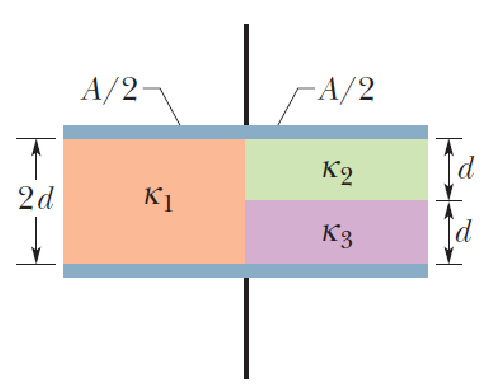
\includegraphics[width=0.5\textwidth]{spho_book_TYS_images/2021SPhO_1.png}
        \label{fig:1}
    \end{figure}
\end{problem}

\begin{solution}
        The system of dielectrics can be considered as 3 separate capacitors. 
        

        \tikzset{every picture/.style={line width=0.75pt}} %set default line width to 0.75pt    
        \begin{center}
        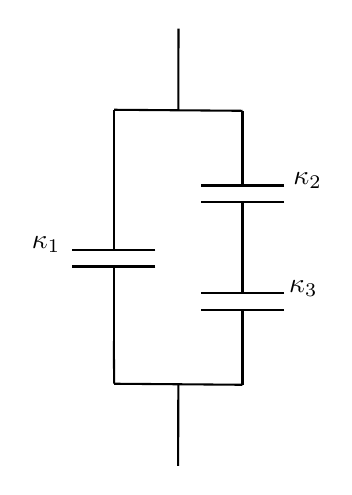
\begin{tikzpicture}[x=0.75pt,y=0.75pt,yscale=-1,xscale=1]
%uncomment if require: \path (0,300); %set diagram left start at 0, and has height of 300

%Shape: Capacitor [id:dp8876925456723114] 
\draw   (96,90.25) -- (96,126.25) (116,134.25) -- (76,134.25) (116,126.25) -- (76,126.25) (96,134.25) -- (96,170.25) ;
%Shape: Capacitor [id:dp7164337300401005] 
\draw   (158,59.25) -- (158,95.25) (178,103.25) -- (138,103.25) (178,95.25) -- (138,95.25) (158,103.25) -- (158,139.25) ;
%Shape: Capacitor [id:dp01288255643149061] 
\draw   (158,111.25) -- (158,147.25) (178,155.25) -- (138,155.25) (178,147.25) -- (138,147.25) (158,155.25) -- (158,191.25) ;
%Straight Lines [id:da5401611279906677] 
\draw    (158,191.25) -- (96.17,190.75) ;
%Straight Lines [id:da7730662393256018] 
\draw    (96.17,190.75) -- (96,170.25) ;
%Straight Lines [id:da1046670903239949] 
\draw    (158,59.25) -- (96.17,58.75) ;
%Straight Lines [id:da9425339678685702] 
\draw    (96,90.25) -- (96,58.75) ;
%Straight Lines [id:da6454401602710205] 
\draw    (127.17,19.7) -- (127.08,59) ;
%Straight Lines [id:da0804701891094548] 
\draw    (127.08,191) -- (127,230.3) ;

% Text Node
\draw (55,118.4) node [anchor=north west][inner sep=0.75pt]    {$\kappa _{1}$};
% Text Node
\draw (181,87.4) node [anchor=north west][inner sep=0.75pt]    {$\kappa _{2}$};
% Text Node
\draw (179,139.4) node [anchor=north west][inner sep=0.75pt]    {$\kappa _{3}$};


\end{tikzpicture}
        \end{center}
        Letting $C_1,C_2$ and $C_3$ be the capacitances of the three capacitors with dielectric constants $\kappa_1$,$\kappa_2$ and $\kappa_3$ respectively,
        \[\text{Total capacitance } C_{eff} = \frac{1}{\frac{1}{C_1}+\frac{1}{C_2+C_3}}\]
        Using $C=\frac{\kappa\epsilon_0A}{d}$ where $A$ is the area of the parallel plates of the capacitor and $d$ is the perpendicular distance between the parallel plates, 
        \[C_1=\frac{\kappa_1\epsilon_0(A/2)}{d}, C_2=\frac{\kappa_2\epsilon_0(A/2)}{d/2} \text{, and } C_3=\frac{\kappa_3\epsilon_0(A/2)}{d/2}\]
        Sub in and simplify: 
        \[C_{eff} = \boxed{\frac{A \kappa _1 \left(\kappa _2+\kappa _3\right) \epsilon _0}{d\left(\kappa _1+2 \left(\kappa _2+\kappa _3\right)\right)}}\]
        % Note to james - just use text environments. I'm not sure I would even put the and in, but if you want to, this is how you do it
\end{solution}

%Question 2
\begin{problem}
    In the rectangle shown, the sides have lengths \qty{5.0}{\cm} and \qty{15}{\cm}, $q1 = \qty{-5.0}{\micro\C}$, and $q2 = \qty{+2.0}{\micro\C}$. 
    \begin{figure}[H]
        \centering
        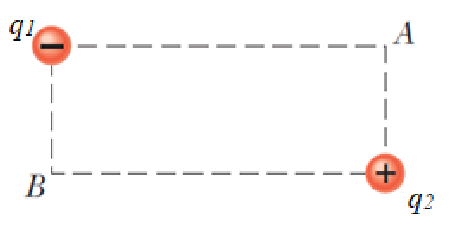
\includegraphics{spho_book_TYS_images/2021SPhO_2.png}
    \end{figure}  
    With  $V = 0$ at infinity, what is the electric potential at
    \begin{subproblemalph}
        \item corner A and \hfill $[1]$
        \item corner B? \hfill $[1]$
        \item How much work is required to move a charge $q3 = \qty{+3.0}{\micro\C}$ from B to A along a diagonal of the rectangle? \hfill $[1]$
        \item Does this work increase or decrease the electric potential energy of the three-charge system? \hfill $[1]$
    \end{subproblemalph}
    Is more, less, or the same work required if q3 is moved along a path that is
    \begin{subproblemalph}
        \setcounter{enumi}{4}
        \item inside the rectangle but not on a diagonal and \hfill $[0.5]$        
        \item outside the rectangle?  \hfill $[0.5]$
    \end{subproblemalph}
\end{problem}

\begin{solution}
    \begin{subsolution}
        \[\phi_A = \frac{1}{4 \pi \varepsilon_0} \left(\frac{q_1}{\qty{0.15}{m}}\frac{q_2}{\qty{0.05}{m}}\right) = \boxed{\qty{59900}{\V}}\text{ (3 s.f.)}\]
    \end{subsolution}
    \begin{subsolution}
        \[\phi_B = \frac{1}{4 \pi \varepsilon_0} \left(\frac{q_1}{\qty{0.05}{m}}\frac{q_2}{\qty{0.15}{m}}\right) = \boxed{\qty{-779000}{\V}}\text{ (3 s.f.)}\]
    \end{subsolution}
    \begin{subsolution}
        \begin{align}
            \text{Work} &= q_3 \left(\phi_A - \phi_B\right) \\
                        & = \boxed{\qty{2.52}{\J}}\text{ (3 s.f.)}
        \end{align}
    \end{subsolution}
    \begin{subsolution}
        If I do positive work on the system, conservation of energy dictates that the electric potential energy increases (assuming all charges are at rest at the end).
    \end{subsolution}
    \begin{subsolution}
    In both cases, the work required is the same since the electric field is conservative.
    \end{subsolution}
    \begin{subsolution}
    (see previous part)
    \end{subsolution}
\end{solution}

\begin{problem}
    The conducting rod shown in the figure has length $L$ and is being pulled along horizontal, frictionless conducting rails at a constant velocity $\vec{v}$. The rails are connected at one end with a metal strip. A uniform magnetic field $\vec{B}$, directed out of the page, fills the region in which the rod moves. Assume that $L = \qty{10}{\cm}$, $v = \qty{5.0}{\m\per\s}$, and $B = \qty{1.2}{\tesla}$. 
    \begin{figure}[H]
        \centering
        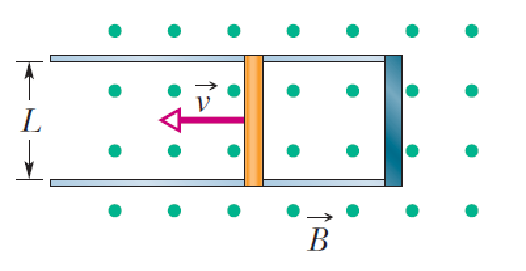
\includegraphics{spho_book_TYS_images/2021SPhO_3.png}
    \end{figure}
    What are the
    \begin{subproblemalph}
        \item magnitude and \hfill [1]
        \item direction (up or down the page) of the emf induced in the rod? \hfill [0.5]
        \item magnitude and \hfill [0.5]
        \item direction of the current in the conducting loop? \hfill [0.5]
    \end{subproblemalph}
    Assume that the resistance of the rod is $\qty{0.40}{\ohm}$ and that the resistance of the rails and metal strip is negligibly small.
    \begin{subproblemalph}
        \setcounter{enumi}{4}
        \item At what rate is thermal energy being generated in the rod? \hfill [1]
        \item What external force on the rod is needed to maintain $\vec{v}$? \hfill [1.5]
        \item At what rate does this force do work on the rod? \hfill [1]
    \end{subproblemalph}
\end{problem}

\begin{solution}
    \begin{subsolution}
        \begin{align}
            \mathcal{E} &= \left|-\frac{\mathrm{d}\phi}{\mathrm{d}t}\right| \\
                        &= \left|-B\frac{\mathrm{d}A}{\mathrm{d}t}\right| \\
                        &= \left|-B L \left|\Vec{v}\right|\right| \\
                        &= \boxed{\qty{0.600}{V}}
        \end{align}
    \end{subsolution}
    \begin{subsolution}
        Use Lenz's Law, B field generated into page means emf induced \boxed{\text{points up}}.
    \end{subsolution}
    \begin{subsolution}
        \[I = \frac{\mathcal{E}}{R} = \boxed{\qty{1.50}{A}}\]
    \end{subsolution}
    \begin{subsolution}
        Based on (ii), current flows \boxed{\text{clockwise}}.
    \end{subsolution}
    \begin{subsolution}
        \[\text{Heat generated} = P = I^2R = \boxed{\qty{0.90}{W}}\]
    \end{subsolution}
    \begin{subsolution}
        To maintain $\Vec{v}$, we need the body to be in equilibrium. Hence
        \[F_{ext} = F_{B} = BIL = \boxed{\qty{0.180}{N}}\]
    \end{subsolution}
    \begin{subsolution}
        \begin{align}
            P &= \frac{\mathrm{d}}{\mathrm{d}t} (F_B x) \\
            &=  F_B \frac{\mathrm{d}x}{\mathrm{d}t} \\
            &= F_B v \\
            &= \boxed{\qty{0.90}{W}}
        \end{align}
        It is the same as the heat generated in the rod, which provides some guarantee of your answer. 
    \end{subsolution}
\end{solution}
\newpage
\begin{problem}
    In the figure shown, after the switch S is closed at time $t = 0$, the emf of the source is automatically adjusted to maintain a constant current $I$ through S.
    \begin{figure}[H]
        \centering
        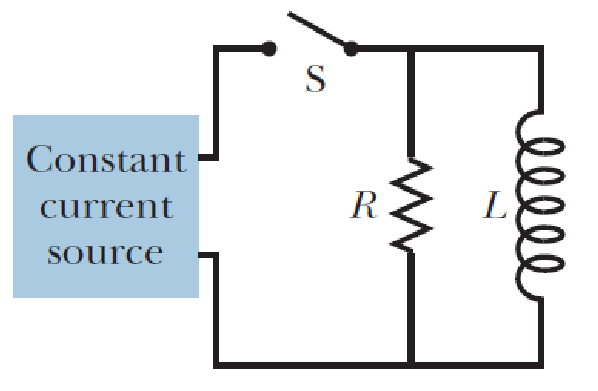
\includegraphics{spho_book_TYS_images/2021SPhO_4.png}
    \end{figure}
    \begin{subproblemalph}
        \item Find the current through the inductor as
a function of time. \hfill $[4]$
        \item At what time is the current through the
resistor equal to the current through the
inductor? \hfill $[1]$
    \end{subproblemalph} 
\end{problem}

\begin{solution}
    \begin{subsolution}
        There is constant current $I$ at S. Thus, current at resistor $I_R = I - I_L$, where $I_L$ is the current at the inductor.
        The inductor's PD equation is: 
        \[V_L = -L \frac{\D I_L}{\D t}\]
        The resistor's PD equation is:
        \[V_R = R I_R\]
        Using voltage loop, 
        \begin{align}
            L \frac{\D I_L}{\D t} &= R I_R \\
            \frac{\D I_L}{\D t} &= \frac{\D(I - I_R)}{\D t} = -\frac{\D I_R}{\D t} \\
            -L \frac{\D I_R}{\D t} &= R I_R \\
            \int \frac{1}{I_R} \D I_R &= -\int \frac{R}{L} \D t \\
            \ln{\frac{I_R}{C}} &= -\frac{R}{L}t
        \end{align}
        for some constant $C$. When $t=0$, $I_R = I$, since all the current flows through the resistor branch. Hence, $C=I$ and:
        \[I_R=I{e}^{-(R/L)t}\]
        \[I_L=\boxed{I\left(1-{e}^{-(R/L)t}\right)}\]
    \end{subsolution}
    \begin{subsolution}
        Equating $I_R$ and $I_L$,
        \begin{align*}
            I{e}^{-(R/L)t}&=I\left(1-{e}^{-(R/L)t}\right)\\
            2I{e}^{-(R/L)t}&=I\\
            -\frac{R}{L}t&=-\ln 2\\
            t&=\boxed{\frac{L}{R}\ln 2}
        \end{align*}
    \end{subsolution}
\end{solution}

\newpage

\begin{problem}
    In the figure shown, a string, tied to a sinusoidal oscillator at P and running over a support at Q, is stretched by a block of mass m. The separation L between P and Q is $\qty{1.20}{\m}$, and the frequency f of the oscillator is fixed at $\qty{120}{\Hz}$. The amplitude of the motion at P is small enough for that point to be considered a node. A node also exists at Q. A standing wave appears when the mass of the hanging block is $\qty{286.1}{\g}$ or $\qty{447.0}{\g}$, but not for any intermediate mass. What is the linear density of the string? \hfill $[6]$
    \begin{figure}[H]
        \centering
        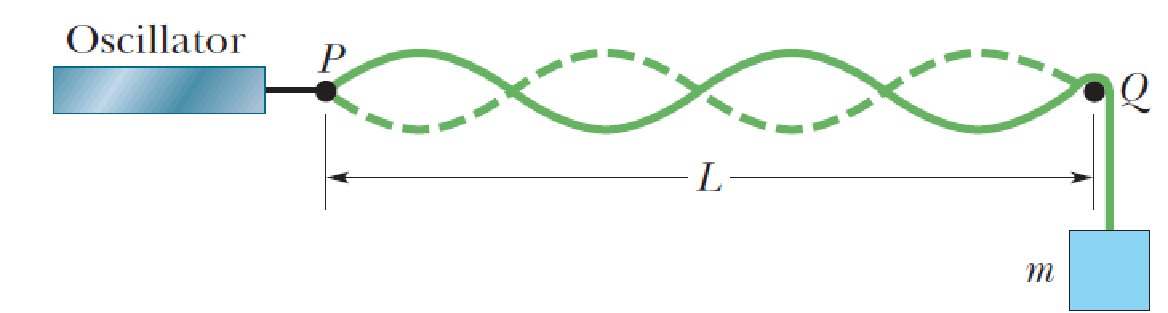
\includegraphics[width=0.8\linewidth]{spho_book_TYS_images/2021SPhO_5.png}
    \end{figure}
\end{problem}

\begin{solution}
    The velocity of a wave in a string is:
    \[v = \sqrt{\frac{T}{\mu}} = \sqrt{\frac{mg}{\mu}} = f\lambda\]
    Since we are provided with two values of m, \(m_1\) and \(m_2\), we check:
    \[\sqrt{\frac{m_1}{m_2}} \approx \frac{4}{5}\]
    Hence:
    \[\frac{\lambda_1}{\lambda_2} \approx \frac{4}{5}\]
    Since the separation L must be \(\frac{n\lambda}{2}\) for some integer \(n\), we conclude that:
    \[L = 2\lambda_1 = \frac{5}{2}\lambda_2\]
    Thus:
    \[\sqrt{\frac{m_1g}{\mu}} = \frac{fL}{2}\]
    Rearranging,
    \[\sqrt{\mu} = \frac{2\sqrt{m_1g}}{fL}\]
    \[\boxed{\mu = \frac{4m_1g}{f^2L^2}}\]
\end{solution}
\newpage
\begin{problem}
    Calculate the minimum kinetic energy an electron must have in order to be constrained within the nucleus, with a typical nuclear radius of $r = \qty{6e-15}{\m}$. Assume that the uncertainty of this electron’s position is equal to the nuclear radius r. Treat the electron relativistically. \hfill $[6]$
\end{problem}
\begin{solution}
    Using Heisenberg's uncertainty principle, the uncertainty in the electron's position $\Delta r$ must be within the nuclear radius $r$:
    \[\Delta p\Delta r \approx \Delta pr = \frac{\hbar}{2}\]
    Approximating $\Delta p$ as the electron's momentum $p$:
    \[\Delta pr \approx pr = \frac{\hbar}{2}\]
    Thus:
    \[p = \frac{\hbar}{2r}\]
    Hence the electron's kinetic energy:
    \begin{equation}
        \begin{split}
            E_k &= E - m_0c^2 \\
            &= \sqrt{p^2c^2+m_0^2c^4} - m_0c^2 \\
            &= \boxed{\sqrt{\frac{\hbar^2c^2}{4r^2}+m_0^2c^4} - m_0c^2} \\
        \end{split}
    \end{equation}
\end{solution}
\newpage
\begin{problem}
    A small $\qty{50}{\g}$ block slides down a frictionless surface through height $h = \qty{20}{\cm}$ and then sticks to a uniform rod of mass $\qty{100}{\g}$ and length \qty{40}{cm}. The rod pivots about point O through angle $\theta$ before momentarily stopping. Find $\theta$. \hfill $[10]$
    \begin{figure}[H]
        \centering
        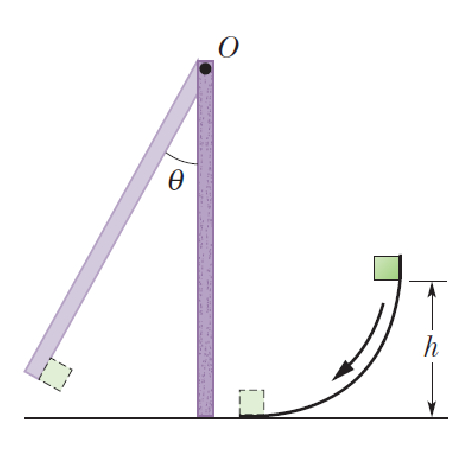
\includegraphics{spho_book_TYS_images/2021SPhO_7.png}
    \end{figure}
\end{problem}
\begin{solution}
    We first consider the collision of the block of mass $m$ and the rod of mass $M$ and length $\ell$:
    \[mgh = \frac{1}{2}mv^2 = \frac{p^2}{2m}\]
    \[p = m\sqrt{2gh}\]
    By conservation of angular momentum $L$:
    \[L = p\ell = m\ell\sqrt{2gh}\]
    We now consider the rotational kinetic energy:
    \[E = \frac{L^2}{2I}\]
    Where $I$ is the moment of inertia:
    \[I = \frac{1}{3}M\ell^2 + m\ell^2\]
    By conservation of energy,
    \begin{equation}
        \begin{split}
            E &= \frac{L^2}{2I} \\
            &= \frac{p^2\ell^2}{2(\frac{1}{3}M\ell^2 + m\ell^2)}\\
            &= \frac{2ghm^2\ell^2}{2\ell^2(\frac{1}{3}M + m)}\\
            &= \frac{ghm^2}{(\frac{1}{3}M + m)}\\
            &= mg(\ell-\ell\cos\theta)+Mg(\frac{\ell}{2}-\frac{\ell}{2}\cos\theta)\\
            &= g\ell(1-\cos\theta)(m+\frac{M}{2})
        \end{split}
    \end{equation}
    Rearranging,
    \[1-\cos\theta = \frac{ghm^2}{g\ell(\frac{1}{3}M + m)(m+\frac{M}{2})}\]
    \[\boxed{\cos\theta = 1-\frac{hm^2}{\ell(\frac{1}{3}M + m)(m+\frac{M}{2})}}\]
\end{solution}
\newpage
\begin{problem}
    The figure shows a reversible cycle through which \qty{1.00}{\mol} of a monoatomic ideal gas is taken. Volume $V_c = 8.00V_b$. Process $bc$ is an adiabatic expansion, with $p_b = 10.0\,\mathrm{atm}$ and $V_b = \qty{1.00e-3}{\cubic\m}$. 
    \begin{figure}[H]
        \centering
        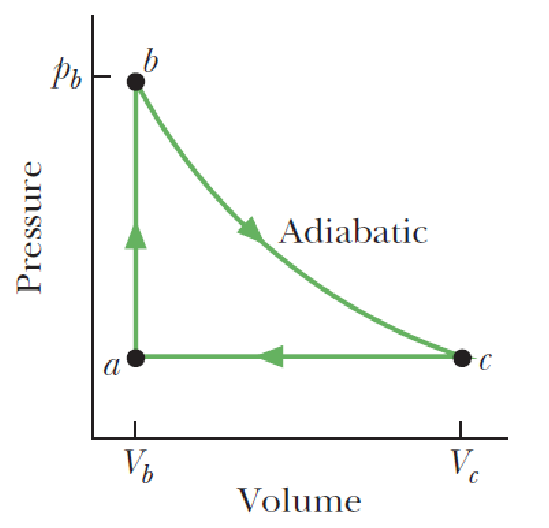
\includegraphics[width=0.5\textwidth]{spho_book_TYS_images/2021SPhO_8.png}
    \end{figure}
    
    For the cycle, find
    \begin{subproblemalph}
        \item the energy added to the gas as heat, \hfill $[3]$
        \item the energy leaving the gas as heat, \hfill $[3]$
        \item the net work done by the gas, and \hfill $[1]$
        \item the efficiency of the cycle. \hfill $[1]$
    \end{subproblemalph}
\end{problem}

\begin{solution}
    \begin{subsolution}
        Firstly, we note that since the gas expands adiabatically along $bc$, letting the pressure at point $c$ be $p_c$,
        \begin{align*}
            p_c V_c^{\gamma}&=p_b V_b^{\gamma}\\
            p_c&=p_b \left(\frac{V_b}{V_c}\right)^{\gamma}
        \end{align*}
        where $\gamma$ is the adiabatic index. For a monoatomic ideal gas, $\gamma=\frac{5}{3}$, so:
        \begin{align*}
            p_c&=p_b \left(\frac{1}{8}\right)^{5/3}\\
            &=\frac{1}{32}p_b
        \end{align*}
        Heat is added to the gas only during process $ab$:
        \begin{align*}
            \Delta Q&=\Delta U - \Delta W\\
            &=\frac{3}{2}p_b V_b - \frac{3}{2}p_c V_b - 0\\
            &=\frac{3}{2}p_b V_b\left(1-\frac{1}{32}\right)\\
            &=\frac{93}{64}p_b V_b\\
            &=\boxed{\qty{1.47e3}{\J}}\text{ (3 s.f.)}
        \end{align*}
    \end{subsolution}
    \begin{subsolution}
        Heat is removed from the gas only during process $ca$:
        \begin{align*}
            \Delta Q&=\Delta U - \Delta W\\
            &=\left(\frac{3}{2}p_cV_b-\frac{3}{2}p_cV_c\right) - \left(-p_c(V_b-V_c)\right)\\
            &=\frac{3}{2}\left(\left(\frac{1}{32}p_b\right)V_b-\left(\frac{1}{32}p_b\right)(8V_b)\right) + \left(\frac{1}{32}p_b\right)(V_b-8V_b)\\
            &=-\frac{35}{64}p_bV_b\\
            &=-\boxed{\qty{554}{\J}}\text{ (3 s.f.)}
        \end{align*}
    \end{subsolution}
    \begin{subsolution}
        After each cycle, the net heat energy input to the gas is:
        \[\frac{93}{64}p_b V_b-\frac{35}{64}p_b V_b=\frac{29}{32}p_b V_b\]
        All of this energy has to become the work done by the gas. Hence,
        \begin{align*}
            W&=\frac{29}{32}p_b V_b\\
            &=\boxed{\qty{918}{\J}}\text{ (3 s.f.)}
        \end{align*}
    \end{subsolution}
    \begin{subsolution}
        The efficiency is:
        \begin{align*}
            \eta&=\frac{W}{Q_h}\\
            &=\frac{\frac{29}{32}p_b V_b}{\frac{93}{64}p_b V_b}\\
            &=\frac{58}{93}\\
            &=\boxed{62.4\%}\text{ (3 s.f.)}
        \end{align*}
    \end{subsolution}
\end{solution}
\newpage
\begin{problem}
    An ideal massless spring with spring constant $k = \qty{10}{\N\per\m}$ and unstretched length $L = \qty{0.5}{\m}$ is attached to point O on axis of a disc. It has a point mass $m = \qty{1}{\kg}$ attached at $L_1 = \qty{0.2}{\m}$ of the unstretched spring. The spring is stretched and the other end is attached to point A on the edge of the disc at $R_0 = \qty{1}{\m}$. The point mass is constrained to move radially only.
    \begin{figure}[H]
        \centering
        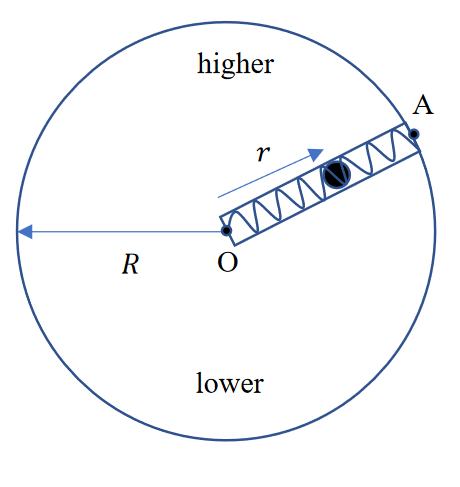
\includegraphics{spho_book_TYS_images/2021SPhO_9.png}
    \end{figure}
    The disc can rotate around the axis at a constant an angular frequency $\omega$. Take $t = \qty{0}{\s}$ when OA is horizontal and A is to the right and the disc is rotating anti-clockwise. Although some air resistance will help the system achieve a steady state, you may assume that air resistance is negligible in your working.
    \begin{subproblemalph}
        \item If the disc is \textbf{horizontal} and $\omega = 0$, derive an expression for the effective spring constant $k_t$ in terms of the given parameters. \hfill $[5]$
        \item If the disc is horizontal and rotating and constant angular velocity $\omega$, derive an expression for $r_0$, the equilibrium position of the mass. \hfill $[5]$
        \item If the disc is at an angle $\varphi = \qty{0.4}{\radian}$ from the horizontal, what is the lowest angular frequency $\omega$ where the point mass can just about reach the edge of the disc at a steady state? \hfill $[5]$
    \end{subproblemalph}
\end{problem}
\begin{solution}
    \begin{subsolution}
        The mass can be modelled as being attached to two strings, with spring constants $k_1$ and $k_2$. Since the restoring force of both springs acts in the same direction (opposite displacement), the effective spring constant:
        \[k_t = k_1 + k_2 = \frac{k}{\frac{L_1}{L}} + \frac{k}{\frac{L-L_1}{L}} = \boxed{\frac{kL^2}{L_1(L-L_1)}}\]
    \end{subsolution}
    \begin{subsolution}
        Taking displacement towards A as positive, equilibrium position is initially $r_0' = L_1$ or $r_0 = L-L_1$ (I feel the question is ambiguous on the orientation of the spring). 
        When rotating at angular velocity $\omega$, forces must be balanced at $r_0 > r_0'$ as the restoring force of the spring acts towards O. Hence:
        \[k_t(r_0-r_0') = mr_0\omega^2\]
        Rearranging,
        \[r_0(k_t-m\omega^2) = k_tr_0'\]
        \[\boxed{r_0 = \frac{k_tr_0'}{k_t-m\omega^2}}\]
    \end{subsolution}
    \begin{subsolution}
        At the lowest point in the rotation, gravity works to pull the mass directly towards the edge. Hence when calculating the lowest angular velocity, we should consider the forces on the mass when it is at its lowest point along the rotation, and set $r_0 = R$. Hence:
        \[k_t(R-r_0')-mg\sin\varphi = mR\omega^2\]
        \[\boxed{\omega = \sqrt{\frac{k_t(R-r_0')-mg\sin\varphi}{mR}}}\]
    \end{subsolution}
\end{solution}
\newpage

\begin{problem}
    Consider Young’s double slit experiment as shown in the below figure (a). Monochromatic light is being used. Further assume that the screen distance $l$ is much larger than the slit separation $d$ (Figure (b))
    \begin{figure}[h]
        \centering
        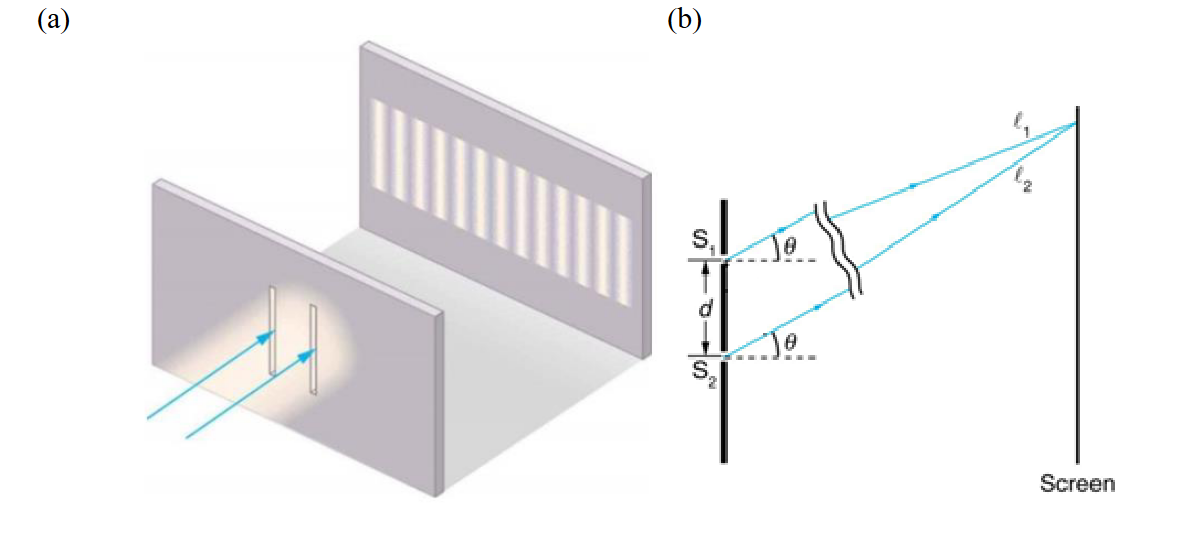
\includegraphics[width = 0.8\textwidth]{spho_book_TYS_images/2021SPhO_10.png}
    \end{figure}
    \begin{subproblemalph}
        \item Under what condition does Young’s experiment show interference pattern? \hfill $[0.5]$
        \item Determine the conditions for obtaining constructive and destructive interference. \hfill $[2]$
        \item Determine the distance $\Delta y$ between adjacent fringes (maxima), assuming that $\theta$ (Figure (b)) is small. \hfill $[2]$
        \item Determine the intensity $I$ of the diffraction pattern’s maxima. You may use \[\sin\alpha + \sin\beta = 2 \cos\frac{1}{2}\left(\alpha-\beta\right)\sin\frac{1}{2}\left(\alpha+\beta\right)\] \hfill $[4.5]$
    \end{subproblemalph}
\end{problem}

\begin{solution}
    \begin{subsolution}
        The light waves entering the slits must be coherent.
    \end{subsolution}
    \begin{subsolution}
        Constructive interference:
        \[d\sin\theta=n\lambda\]
        Destructive interference:
        \[d\sin\theta=\left(n+\frac{1}{2}\right)\lambda\]
        where $n$ is some integer.
    \end{subsolution}
    \begin{subsolution}
        For small $\theta$, $\sin \theta\approx \frac{y}{l}$, where $y$ is the distance from the central maxima. Hence, for 2 adjacent fringes:
        \begin{align*}
            d\cdot \frac{\Delta y}{l}&=\lambda\\
            \Delta y&=\frac{\lambda l}{d}
        \end{align*}
    \end{subsolution}
    \begin{subsolution}
        If we let the light wave reaching the screen from one of the slits to be described by \(E=E_0\sin(\omega t)\), then the other wave from the other slit is \(E=E_0\sin\left(\omega t+\frac{2\pi d\sin\theta}{\lambda}\right)\), since the phase difference between the 2 waves is \(\frac{2\pi d\sin\theta}{\lambda}\). Hence, adding up the waves:
        \begin{align*}
            E_{\mathrm{total}}&=E_0\sin(\omega t)+E_0\sin\left(\omega t+\frac{2\pi d\sin\theta}{\lambda}\right)\\
            &=2E_0\cos\frac{1}{2}\left(\frac{2\pi d\sin\theta}{\lambda}\right)\sin\frac{1}{2}\left(2\omega t+\frac{2\pi d\sin\theta}{\lambda}\right)\\
            &=2E_0\cos\left(\frac{\pi d\sin\theta}{\lambda}\right)\sin\left(\omega t+\frac{\pi d\sin\theta}{\lambda}\right)
        \end{align*}
        The combined amplitude of the wave is therefore:
        \[E_{\mathrm{total},0}=2E_0\cos\left(\frac{\pi d\sin\theta}{\lambda}\right)\]
        If we let the initial intensity of light be $I_0=kE_0^2$ and the final intensity of light be $I_t=kE_{\mathrm{total},0}^2$ for some constant $k$, we get:
        \[I_t=\boxed{4I_0\cos^2\left(\frac{\pi d\sin\theta}{\lambda}\right)}\]
    \end{subsolution}
\end{solution}
